\heada{MESH}{ANGLe}
\hspace{1.0cm} {{ angl                  \hfill}} \\{\smallskip}
\hspace{1.4cm} {{ node1,ngen1,angl(node1) \hfill}} \\{\smallskip}
\hspace{1.4cm} {{ node2,ngen2,angl(node2) \hfill}} \\{\smallskip}
\hspace{1.4cm} {{ <etc,,terminate with blank record> \hfill}}
\headb

The {\tt ANGL}e command is used to specify angles (degrees)
for sloping nodal boundary conditions as shown in Fig. \ref{angf1}.
For each node \texttt{I} to be
specified a record is entered with the following information:

\begin{center}
\begin{tabular}{r l}
\it node       &-- the number of the I-node to be specified \\
\it ngen       &-- the increment to the next node, if \\
               &\quad generation is used, otherwise 0. \\
\it angl(node) &-- value of angle new 1-coordinate makes \\
               & \quad with x(1,node).
\end{tabular}
\end{center}
When generation is performed, the node number sequence
will be (for {\it node1-node2} sequence shown above):

\begin{center}
{\it node1, node1+ngen1, node1+2$\times$ngen1, .... , node2}
\end{center}

\noindent
The values for each angle generated will be a linear interpolation
between {\it node1} and {\it node2}.

\begin{figure}[ht!]
\begin{center}
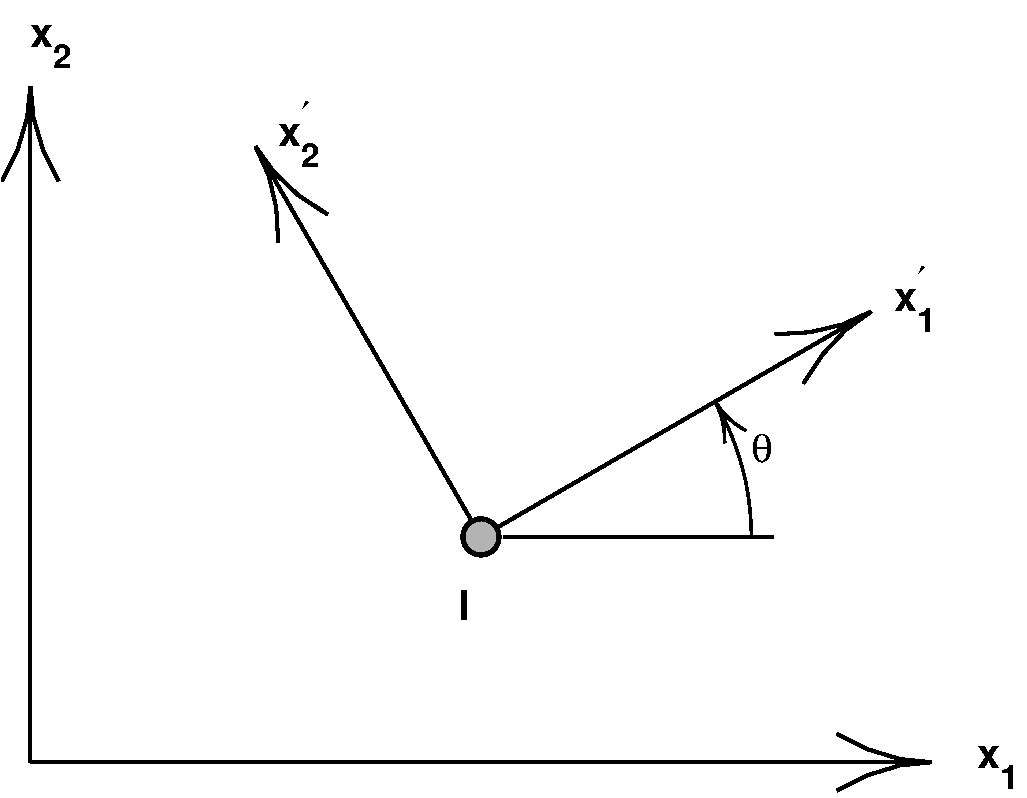
\includegraphics[width=3.5in]{../lmesh/angcor}
\caption{Coordinate rotation for nodes. \label{angf1} }
\end{center}
\end{figure}

The degrees-of-freedom associated with the sloping
boundary may differ from element to element as described in
the element manuals.  The default will be the first two
degrees-of-freedom (2 and 3-D problems) which are affected by the sloping
condition.  Both force and displacement values will be
assumed to be given in the rotated frame. To activate the rotated
boundary condition use the {\tt BOUN}dary-, {\tt FORC}e-, 
{\tt DISP}lacement- etc. command.

Angle conditions may also be specified using the {\tt EANG}le and {\tt CANG}le
commands.
\pagebreak

\noindent{\bf{Example: ANGLe}}

As an example consider a problem in which degrees of freedom are to be defined
relative to sloping axes.  The statements
\begin{verbatim}
       ANGLe
         1 5 30
        21 0 30

\end{verbatim}
will define the $x_1^\prime$ axis to make an angle of $30^o$ with the $x_1$
axis for nodes 1, 6, 11,16 and 21.  After this command, the first two
degrees of freedom will be in the $x_1^\prime$ and $x_2^\prime$ directions,
respectively.  Also, any specified boundary restraints, forces or displacements
will also be with respect to the $30^o$ rotated axes.
\vfil\eject
